\newcommand{\sourcename}{Fast Response Example}
\newcommand{\analysisid}{2018_01_01_Fast_Response_Example}
\newcommand{\gfurate}{/data/condor_builds/users/efried/FastResponseAnalysis/trunk/2018_01_01_Fast_Response_Example/GFU_rate_plot.png}
\newcommand{\reportdate}{2020-08-18}
\newcommand{\skymap}{/data/condor_builds/users/efried/FastResponseAnalysis/trunk/2018_01_01_Fast_Response_Example/2018_01_01_Fast_Response_Exampleunblinded_skymap.png}
\newcommand{\skymapzoom}{/data/condor_builds/users/efried/FastResponseAnalysis/trunk/2018_01_01_Fast_Response_Example/2018_01_01_Fast_Response_Exampleunblinded_skymap_zoom.png}
\newcommand{\limitdNdE}{/data/condor_builds/users/efried/FastResponseAnalysis/trunk/2018_01_01_Fast_Response_Example/central_90_dNdE.png}
\newcommand{\muonfilter}{/data/condor_builds/users/efried/FastResponseAnalysis/trunk/2018_01_01_Fast_Response_Example/MuonFilter_13_plot.png}
\newcommand{\Lfilter}{/data/condor_builds/users/efried/FastResponseAnalysis/trunk/2018_01_01_Fast_Response_Example/OnlineL2Filter_17_plot.png}
\newcommand{\badnessplot}{/data/condor_builds/users/efried/FastResponseAnalysis/trunk/2018_01_01_Fast_Response_Example/badness_plot.png}
\newcommand{\tsd}{No background TS distribution}
\newcommand{\upperlim}{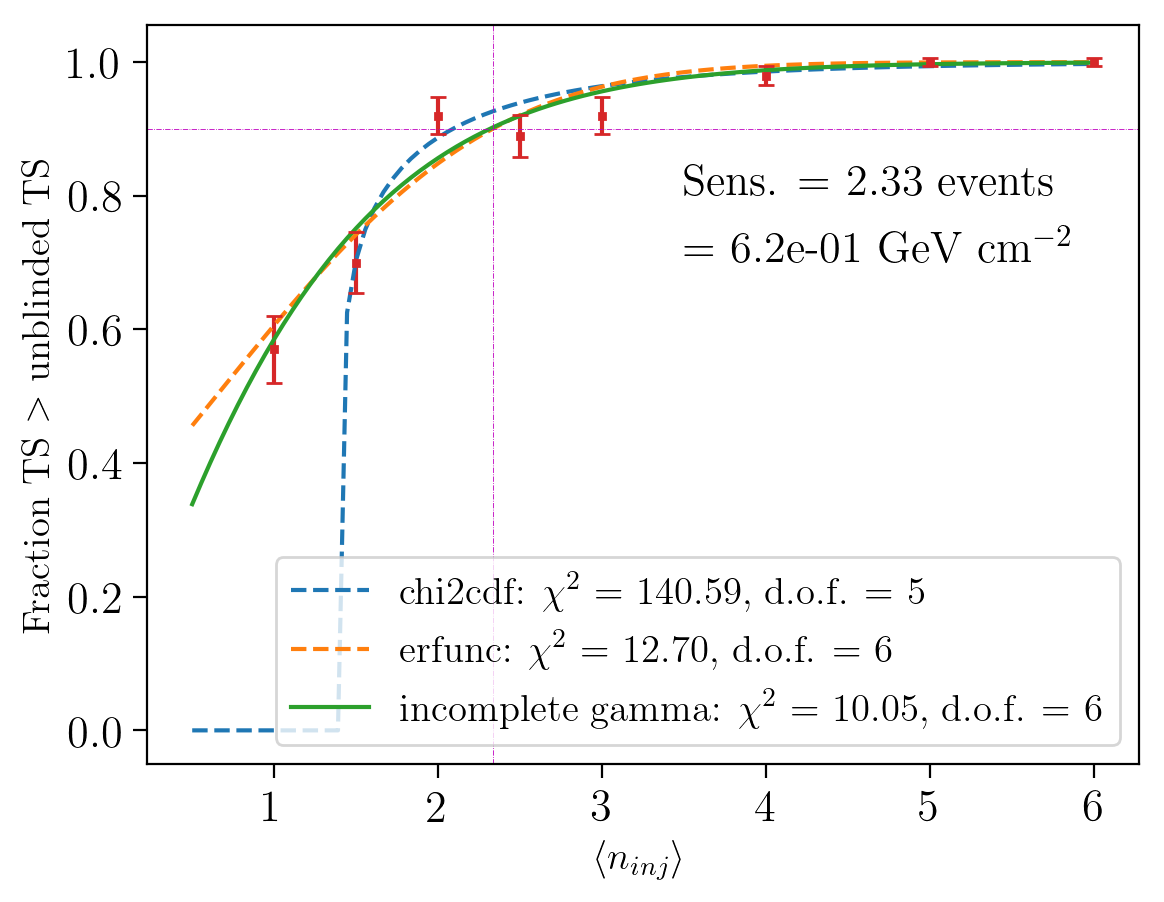
\includegraphics[width=0.9\textwidth]{/data/condor_builds/users/efried/FastResponseAnalysis/trunk/2018_01_01_Fast_Response_Example/upper_limit_distribution.png}}
\newcommand{\nsscan}{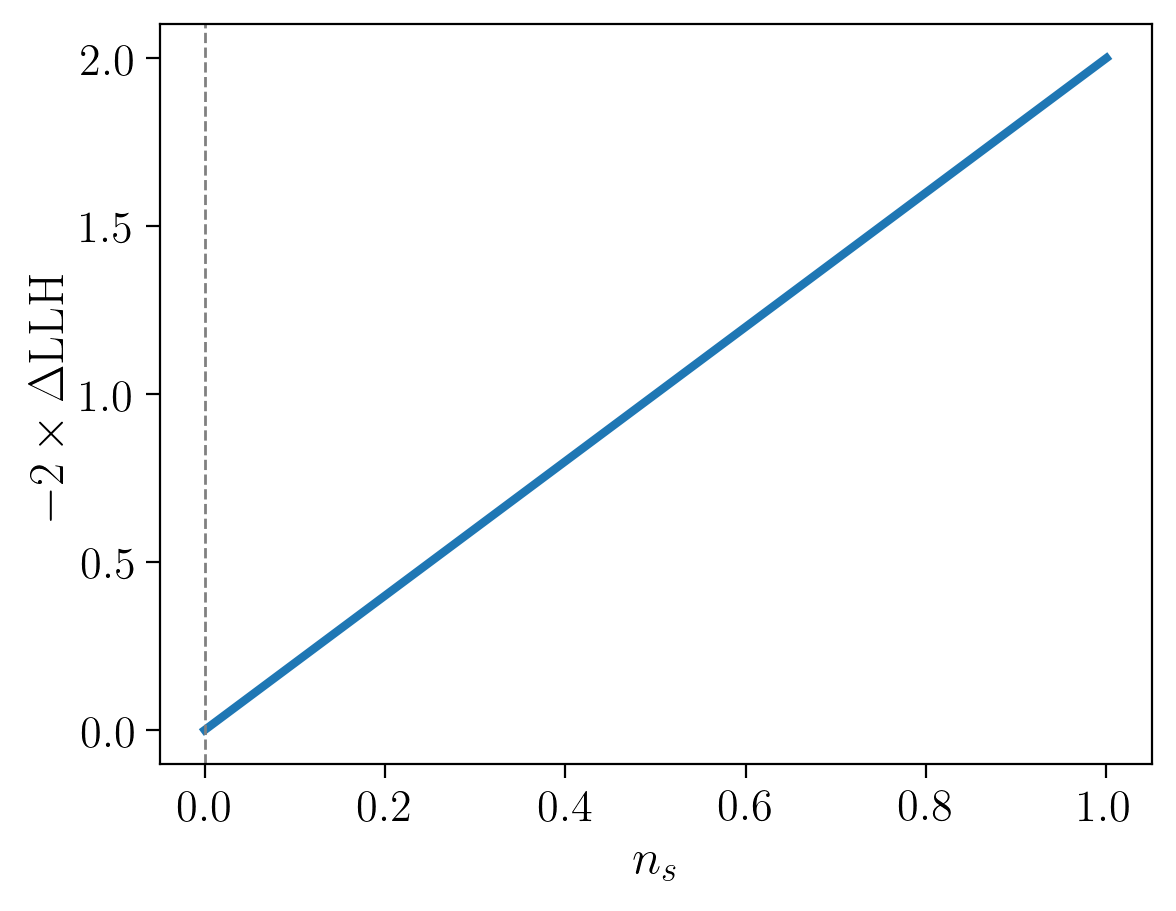
\includegraphics[width=0.9\textwidth]{/data/condor_builds/users/efried/FastResponseAnalysis/trunk/2018_01_01_Fast_Response_Example/llh_ns_scan.png}}
\newcommand{\obsdate}{2018-01-01 -- 2018-01-02}
\newcommand{\multiplicity}{/data/condor_builds/users/efried/FastResponseAnalysis/trunk/2018_01_01_Fast_Response_Example/IN_ICE_SIMPLE_MULTIPLICITY_plot.png}
\newcommand{\survivialfunctionplot}{}
\newcommand{\backgroundpdfplot}{}
\newcommand{\sourcetable}{
\begin{longtable}{ll}
\hline
Source Name & Fast Response Example\\
Trigger Time & 2018-01-02 00:00:00.000 (MJD=58120.000000)\\
Start Time & 2018-01-01 12:00:00.000 (Trigger-43200.0s)\\
Stop Time & 2018-01-02 12:00:00.000 (Trigger+43200.0s)\\
Time Window & 86400.0s\\
\hline
\end{longtable}}
\newcommand{\skylabtable}{
\begin{longtable}{ll}
\hline
Skylab Version & 2.7.2\\
IceTray Path & ['/data/condor\_builds/users/efried/icerec/build\_realtime/lib/icecube/icetray']\\
Created by & i3home/efried\\
Dataset Used & gfu online/version-001-p01/\\
Dataset details & Real-time Gamma-Ray Follow-Up (GFU) Sample with leap second bug fix and official\\
 & neutrino sources format.\\
\hline
\end{longtable}}
\newcommand{\runtimetable}{
\begin{longtable}{lllll}
\hline
Run & Start Time & Stop Time & Duration & Livetime\\ \hline
130484 & 2018-01-01 00:40:35 & 2018-01-01 05:44:15 & 5:03:40 & 0.0s\\
130485 & 2018-01-01 05:45:45 & 2020-08-18 20:24:33 & 23054:38:48 & 86400.0s\\
130486 & 2018-01-01 05:48:54 & 2020-08-18 20:24:33 & 23054:35:39 & 86400.0s\\
130487 & 2018-01-01 05:51:29 & 2018-01-01 09:56:54 & 4:05:24 & 0.0s\\
130488 & 2018-01-01 09:58:06 & 2018-01-01 17:57:07 & 7:59:01 & 21427.0s\\
130489 & 2018-01-01 17:57:07 & 2018-01-02 01:57:40 & 8:00:33 & 28833.0s\\
130490 & 2018-01-02 01:57:40 & 2018-01-02 09:58:00 & 8:00:20 & 28820.0s\\
130491 & 2018-01-02 09:58:00 & 2018-01-02 17:58:22 & 8:00:22 & 7320.0s\\
130492 & 2018-01-02 17:59:53 & 2018-01-03 01:59:27 & 7:59:33 & 0.0s\\
\hline
\end{longtable}}
\newcommand{\runstatustable}{
\begin{longtable}{lllllll}
\hline
Run & Status & Light & Filter Mode & Run Mode & OK & GFU\\ \hline
130484 & FAIL & dark & PhysicsFiltering & PhysicsTrig & NotOK & 119\\
130485 & FAIL & dark & PhysicsFiltering & PhysicsTrig & NotOK & 0\\
130486 & FAIL & dark & PhysicsFiltering & PhysicsTrig & NotOK & 0\\
130487 & FAIL & dark & PhysicsFiltering & PhysicsTrig & NotOK & 101\\
130488 & SUCCESS & dark & PhysicsFiltering & PhysicsTrig & OK & 182\\
130489 & SUCCESS & dark & PhysicsFiltering & PhysicsTrig & OK & 198\\
130490 & SUCCESS & dark & PhysicsFiltering & PhysicsTrig & OK & 181\\
130491 & SUCCESS & dark & PhysicsFiltering & PhysicsTrig & OK & 179\\
130492 & SUCCESS & dark & PhysicsFiltering & PhysicsTrig & OK & 192\\
\hline
\end{longtable}}
\newcommand{\livetime}{259,200.0}
\newcommand{\ontimetable}{
\begin{longtable}{ll}
\hline
Access Method & database\\
Stream & \texttt{neutrino17}\\
Query Time & 2020-08-18 18:24:33\\
Start Time & 2018-01-01 00:40:35\\
Stop Time & 2018-01-03 01:59:27\\
\hline
\end{longtable}}
\newcommand{\event}{[None]}\newcommand{\results}{
\begin{longtable}{ll}
\hline
$n_s$ & 0.000\\
$TS$ & -0.000\\
$p-value$ & 1.0000\\
\hline
\end{longtable}}
